\subsection{To-do list} \label{To-do list}
%\begin{figure}[H]
%	\centering
%	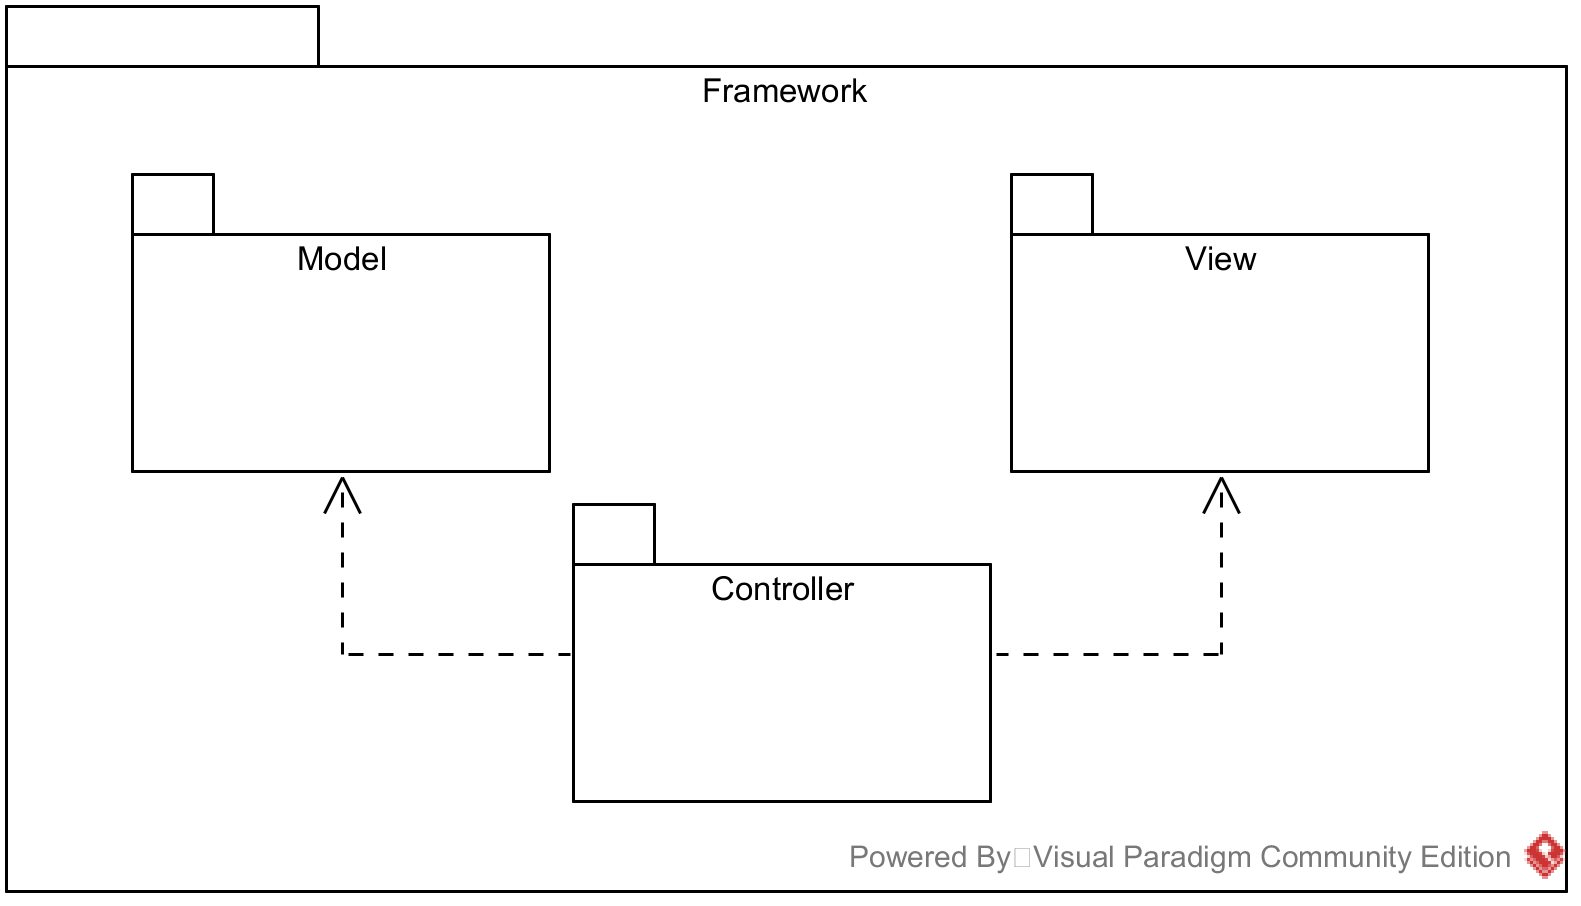
\includegraphics[width=15cm]{./diagrammi/framework.png}
%	\caption{Componente Framework}
%\end{figure}
\glossario{TodoList} è il package base per la prima delle due demo. Come il framework segui il design pattern MVC ed è quindi composto dai package Model, View e Controller.

\setclass{TodoList::Model}
\subsubsection[::Model]{\class} \label{\class}
%\begin{figure}[H]
%	\centering
%	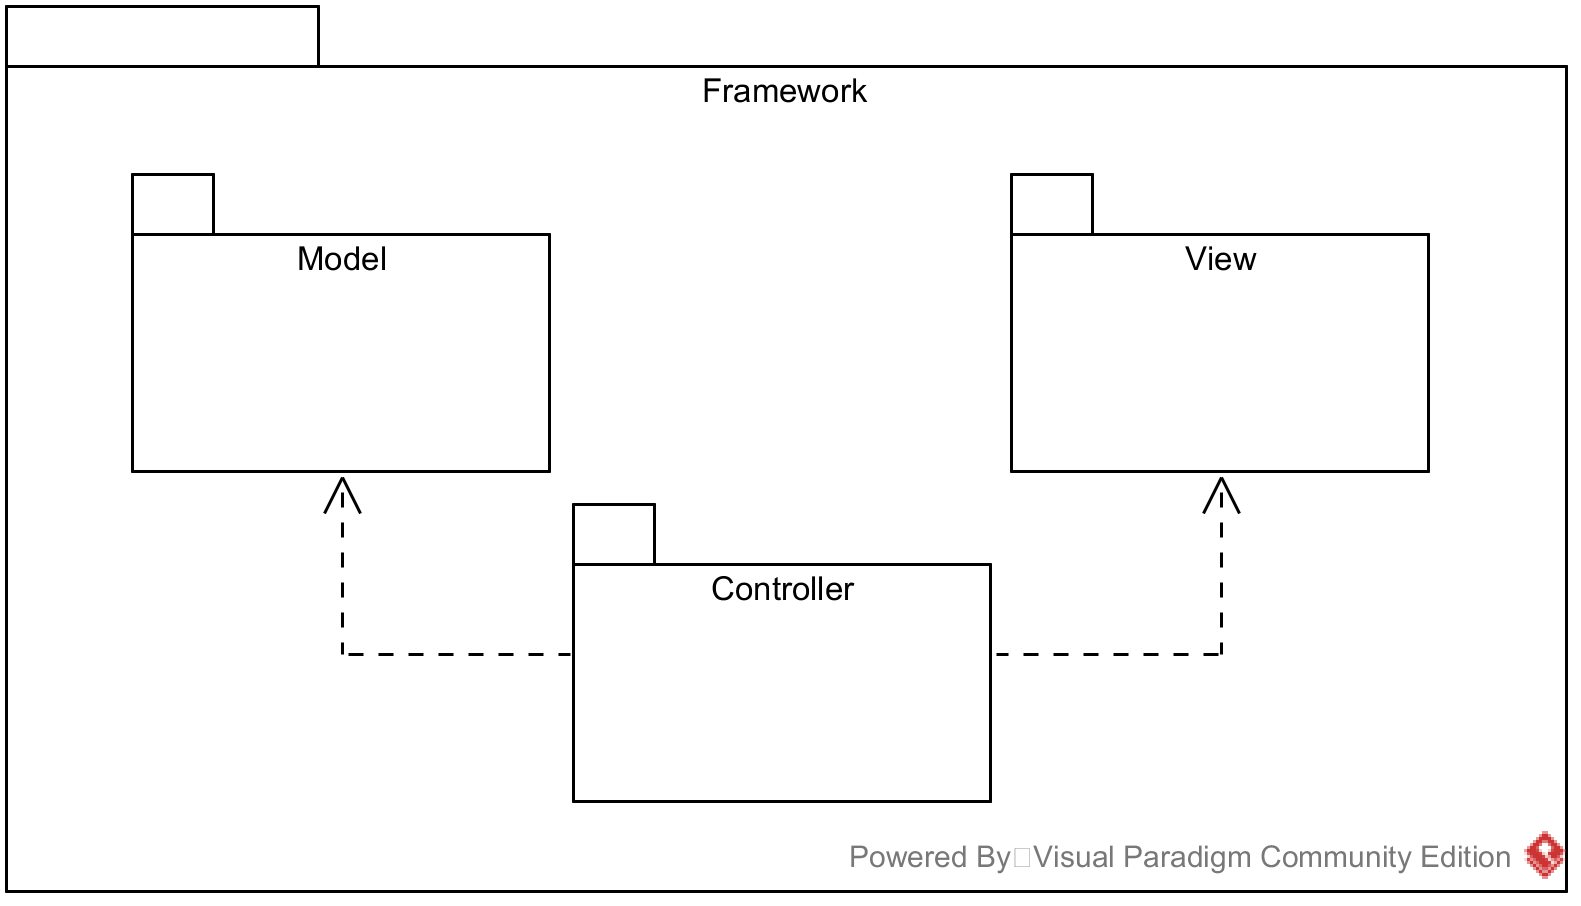
\includegraphics[width=15cm]{./diagrammi/framework.png}
%	\caption{Componente Framework}
%\end{figure}
Il package Model contiene i dati della To-do list ed è composo a sua volta dal package ItemsStore.

\setclass{TodoList::Model::ItemsStore}
\subparagraph[::ItemStore]{\class}\mbox{}\\ \label{\class}
%\begin{figure}[H]
%	\centering
%	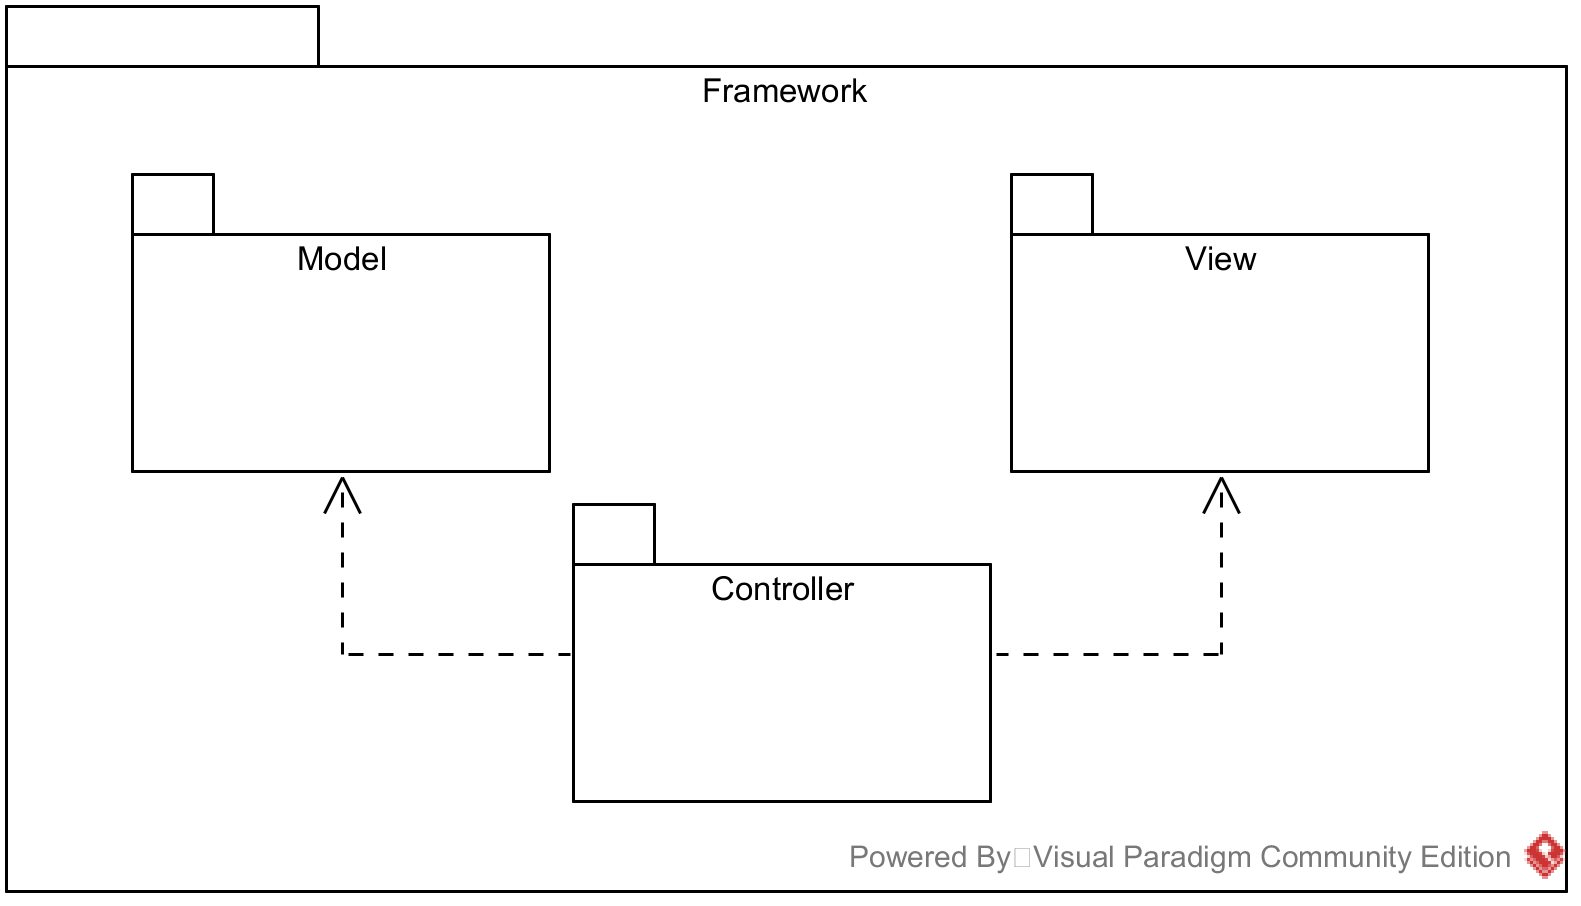
\includegraphics[width=15cm]{./diagrammi/framework.png}
%	\caption{Componente Framework}
%\end{figure}
\textbf{Descrizione:}
ItemStore implementa la classe BubbleMemory e gestisce i dati della To-do list.

\textbf{Utilizzo:}
Viene utilizzata per gestire gli elementi della To-do list.

\textbf{Classi ereditate:}
\begin{itemize}
	\item \code{BubbleMemory}.
\end{itemize}

\textbf{Attributi:}
\begin{itemize}
	\item \field{-items: Object[]}: array contenente gli elementi della lista;
	\item \field{-completed: Object[]}: array contenente gli elementi completati della lista.
\end{itemize}

\textbf{Metodi:}
\begin{itemize}
	\item \method{+ItemsStore()}: costruttore della classe, crea i due array vuoti items e completed;
	\item \method{-addItems(text:object)}: aggiunge un elemento alla lista;
		\begin{itemize}
			\item \param{text:object}: elemento da aggiungere alla lista.
		\end{itemize}
	\item \method{-removeItems(id:string)}: rimuove l'elemento identificato da id dalla lista;
		\begin{itemize}
			\item \param{id:string}: id dell'oggetto da rimuovere.
		\end{itemize}
	\item \method{-completeItems(id:string)}: indica come completato l'elemento id;
		\begin{itemize}
			\item \param{id:string}: id dell'oggetto da indicare come completato.
		\end{itemize}
	\item \method{+getItems():object[]}: restituisce tutti gli elementi della lista;
	\item \method{+GetCompleted():object[]}: restituiscce tutti gli elementi completati della lista;
	\item \method{+handleActions(action:object)}: effettua l'azione richiesta.
		\begin{itemize}
			\item \param{action:object}: azione che si vuole venga effettuata, può essere di tre tipi:
			\begin{itemize}
				\item ADD\_ITEM: indica la richiesta di aggiunta di un oggetto;
				\item REMOVE\_ITEM: indica la richiesta di rimozione di un oggetto;
				\item COMPLETE\_ITEM: indica la richiesta di indicare come completato un oggetto.
			\end{itemize}
		\end{itemize}
\end{itemize}

\setclass{TodoList::View}
\subsubsection[::View]{\class} \label{\class}
%\begin{figure}[H]
%	\centering
%	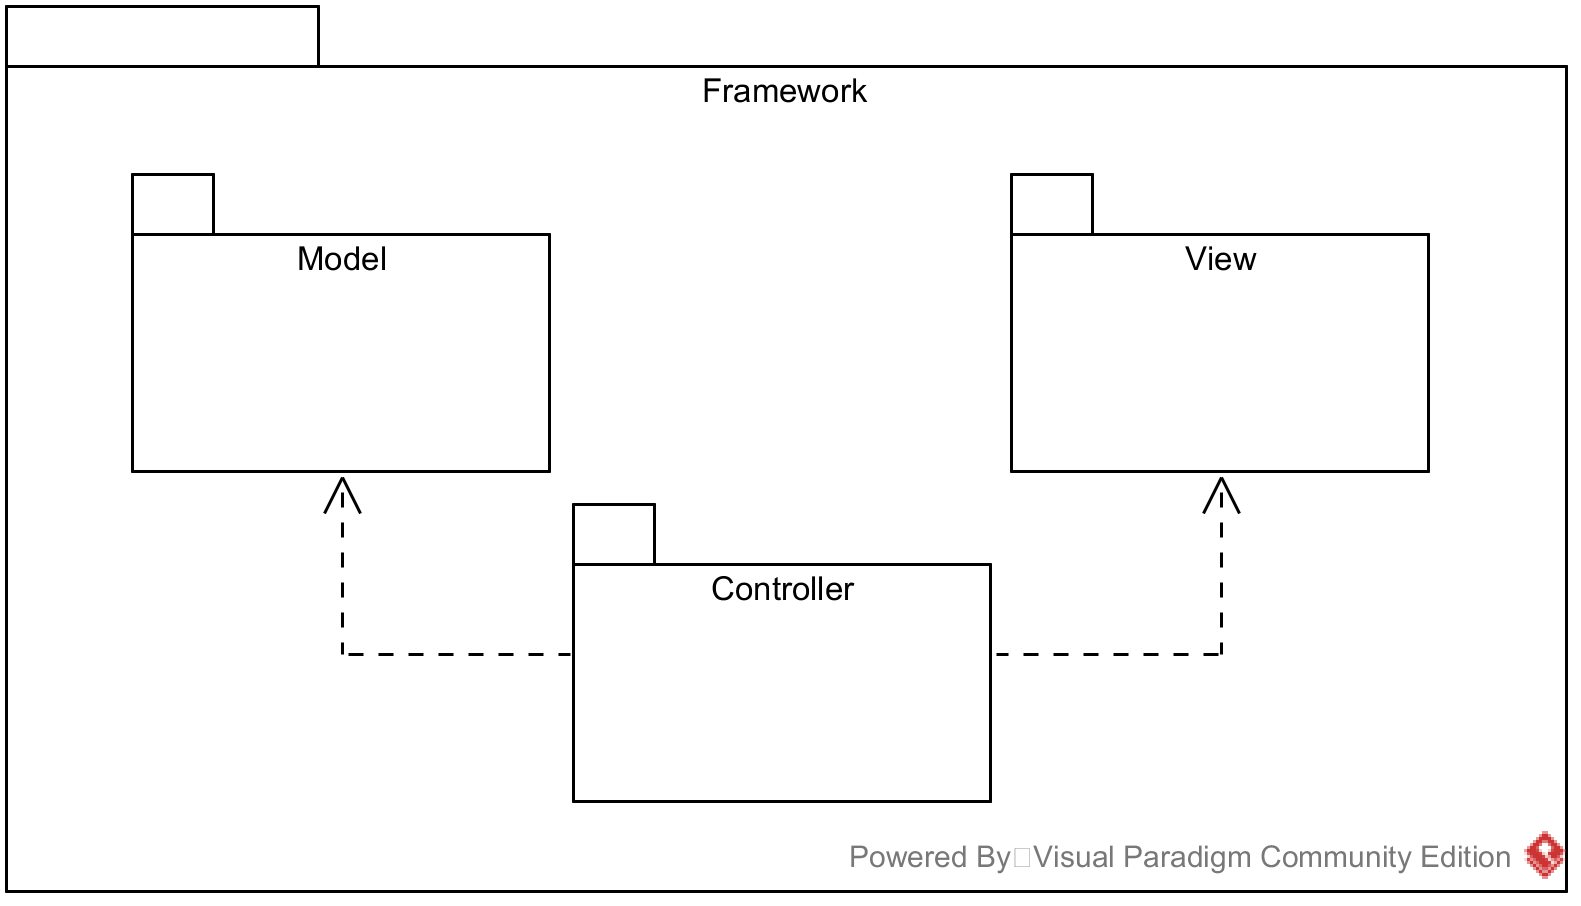
\includegraphics[width=15cm]{./diagrammi/framework.png}
%	\caption{Componente Framework}
%\end{figure}
Il package View si occupa di gestire la parte grafica della To-do list, ed è composto dal package ListItems.

\setclass{TodoList::View::ListItems}
\paragraph[::ListItems]{\class}\mbox{}\\ \label{\class}
%\begin{figure}[H]
%	\centering
%	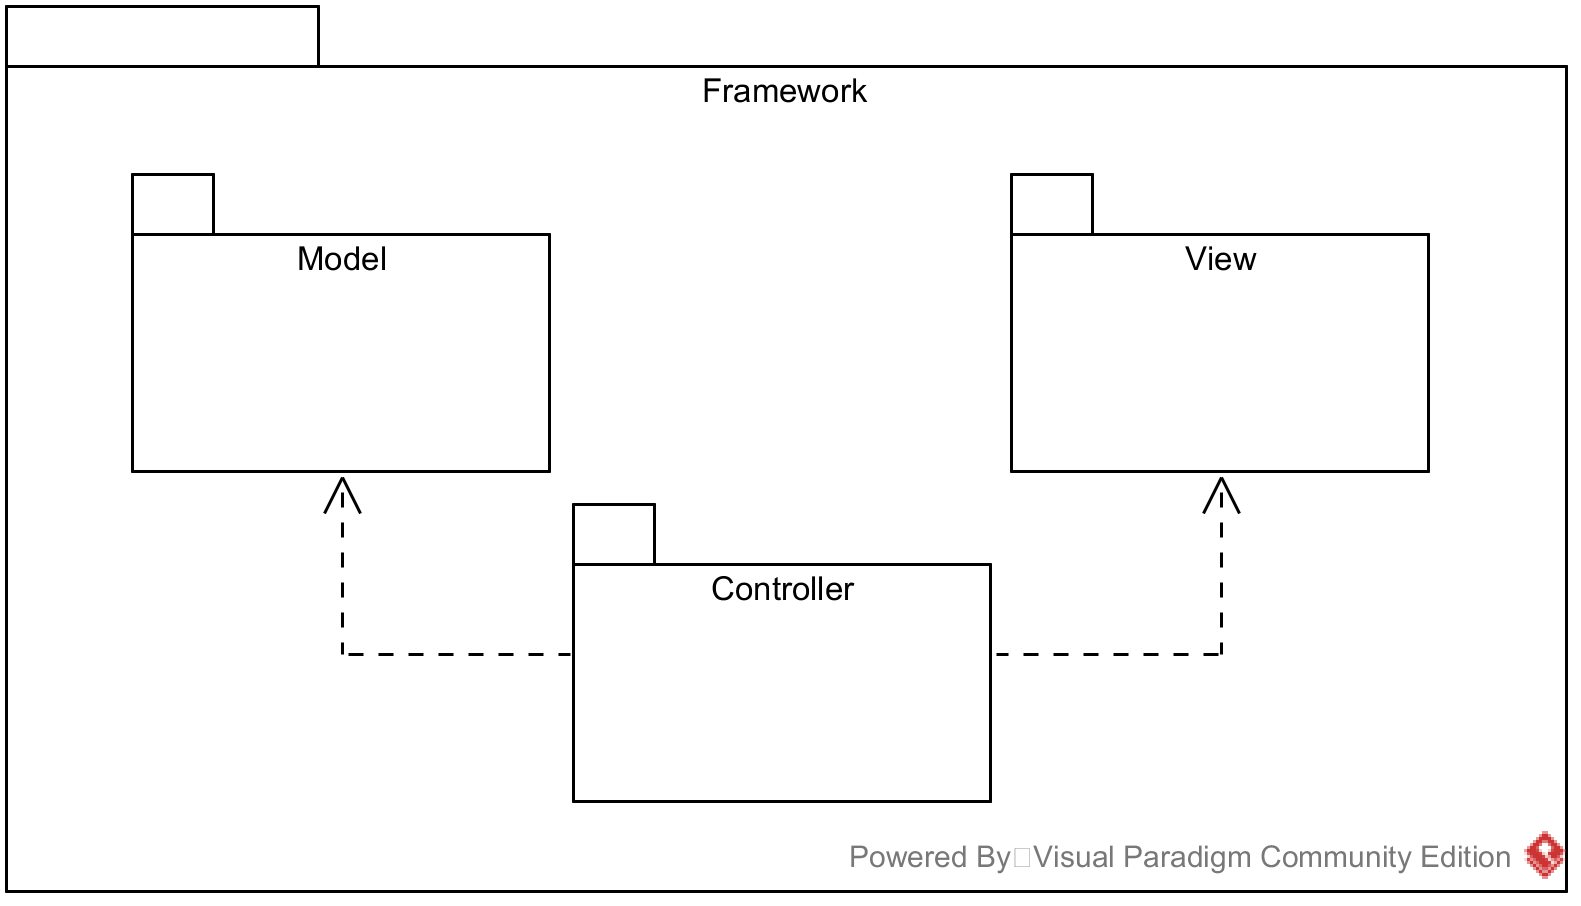
\includegraphics[width=15cm]{./diagrammi/framework.png}
%	\caption{Componente Framework}
%\end{figure}
Il package ListItems è composto dalle due classi listItemContainer e listItem. Gestisce la visualizzazione della lista degli elementi della To-do list.

\setclass{TodoList::View::ListItems::listItem}
\subparagraph[::listItem]{\class}\mbox{}\\ \label{\class}
%\begin{figure}[H]
%	\centering
%	\includegraphics[width=15cm]{./diagrammi/demo/todo-list/listitem.png}
%	\caption{Componente Framework}
%\end{figure}
\textbf{Descrizione:}
Questa classe rappresenta gli elementi della To-do list.

\textbf{Utilizzo:}
Viene utilizzata per riempire la To-do list.

\textbf{Classi ereditate:}
\begin{itemize}
	\item \code{React.Component};
	\item \code{Framework::View::GUI::CheckBox}.
\end{itemize}

\textbf{Attributi:}
\begin{itemize}
	\item \field{-props: Object[]}: array contenente le proprietà di un elemento della lista.
\end{itemize}

\textbf{Metodi:}
\begin{itemize}
	\item \method{+ListItem(props: Object[])}: costruttore della classe, assegna le proprietà:
	\begin{itemize}
		\item \param{props: Object[]}: array contenente le proprietà della classe.
	\end{itemize}
	\item \method{+render(): React.Component}: renderizza il componente.
\end{itemize}

\setclass{TodoList::View::ListItems::listItemContainer}
\subparagraph[::listItemContainer]{\class}\mbox{}\\ \label{\class}
%\begin{figure}[H]
%	\centering
%	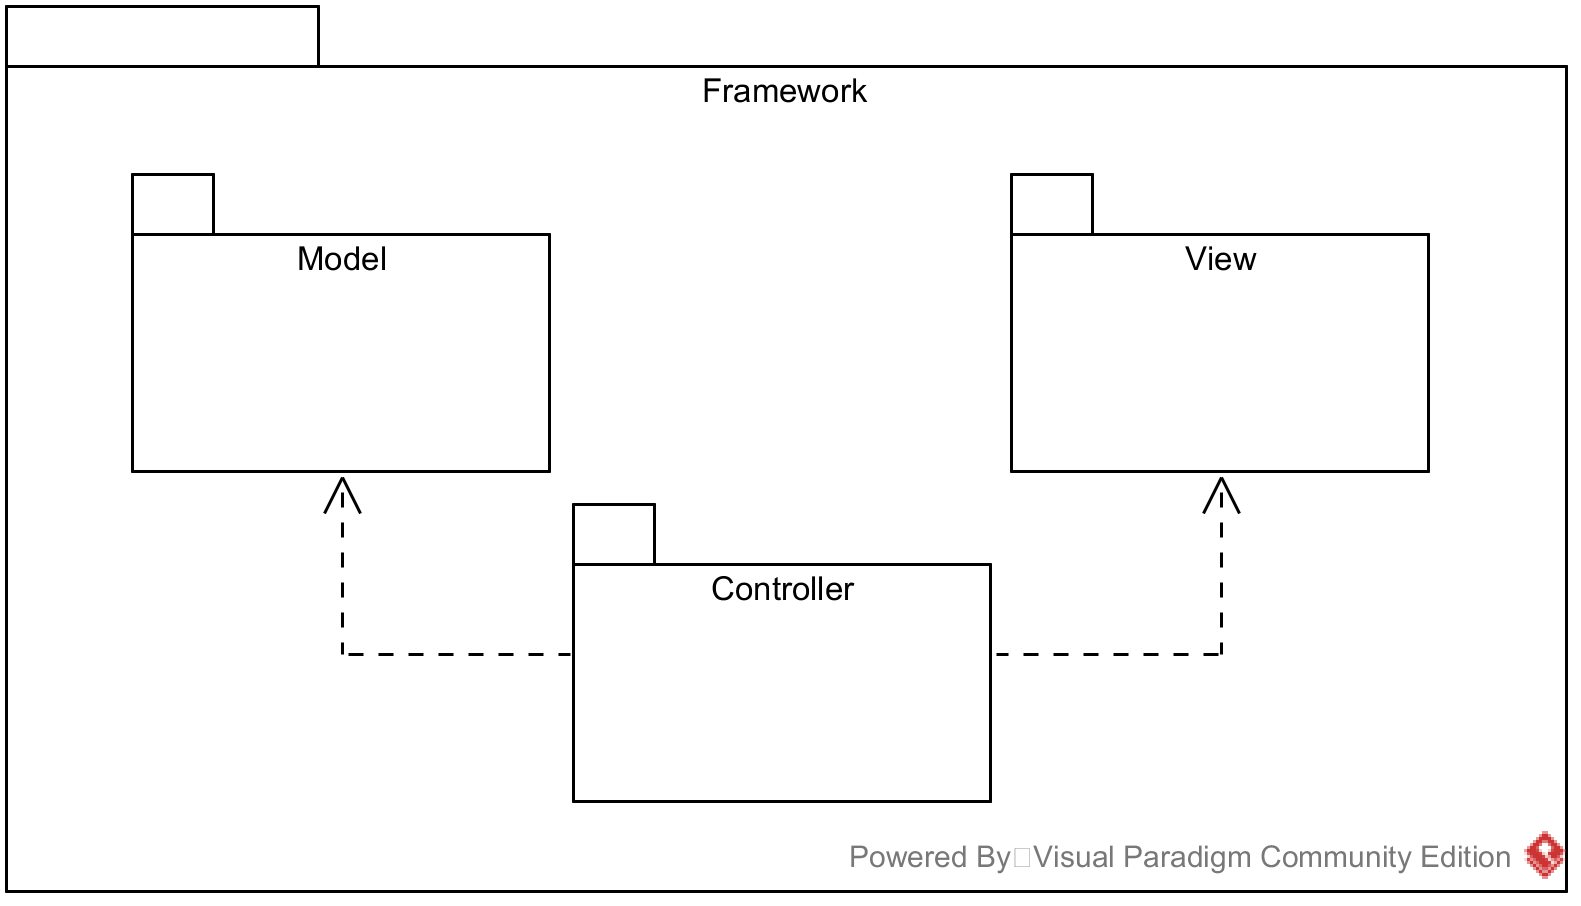
\includegraphics[width=15cm]{./diagrammi/framework.png}
%	\caption{Componente Framework}
%\end{figure}
\textbf{Descrizione:}
Questa classe rappresenta il contenitore degli elementi della To-do list.

\textbf{Utilizzo:}
Viene utilizzata per visualizzare gli elementi della To-do list, fornendo all'utente la possibilità di interagire con la lista.

\textbf{Classi ereditate:}
\begin{itemize}
	\item \code{React.Component};
\end{itemize}

\textbf{Attributi:}
\begin{itemize}
	\item \field{-items: object[]}: array contenente gli elementi della lista;
	\item \field{-completed: object[]}: array contenente gli elementi completati della lista.
\end{itemize}

\textbf{Metodi:}
\begin{itemize}
	\item \method{+ListItemContainer()}: costruttore della classe, crea la lista recuperando i dati da TodoList::Model::ListItems::ItemsStore;
	\item \method{+processInput()}: costruisce la lista di listItem;
	\item \method{+componentWillMount()}: ricarica la lista quando viene effettuata una modifica;
	\item \method{+handleComplete(event:Object)}: comunica al controller di completare un elemento della lista;
		\begin{itemize}
			\item \param{event:Object}: parametro necessario ad evitare il refresh della pagina. 
		\end{itemize}
	\item \method{+handleSubmit(event:Objecct)}: comunica al controller di aggiungere un elemento alla lista;
		\begin{itemize}
			\item \param{event:Object}: parametro necessario ad evitare il refresh della pagina.
		\end{itemize}
	\item \method{+handleRemove(event:Object)}: comunica al controller di rimuovere un elemento dalla lista;
		\begin{itemize}
			\item \param{event:Object}: parametro necessario ad evitare il refresh della pagina.
		\end{itemize}
	\item \method{+render(): React.Component}: renderizza il componente.
\end{itemize}

\setclass{TodoList::Controller}
\subsubsection[::Controller]{\class} \label{\class}
%\begin{figure}[H]
%	\centering
%	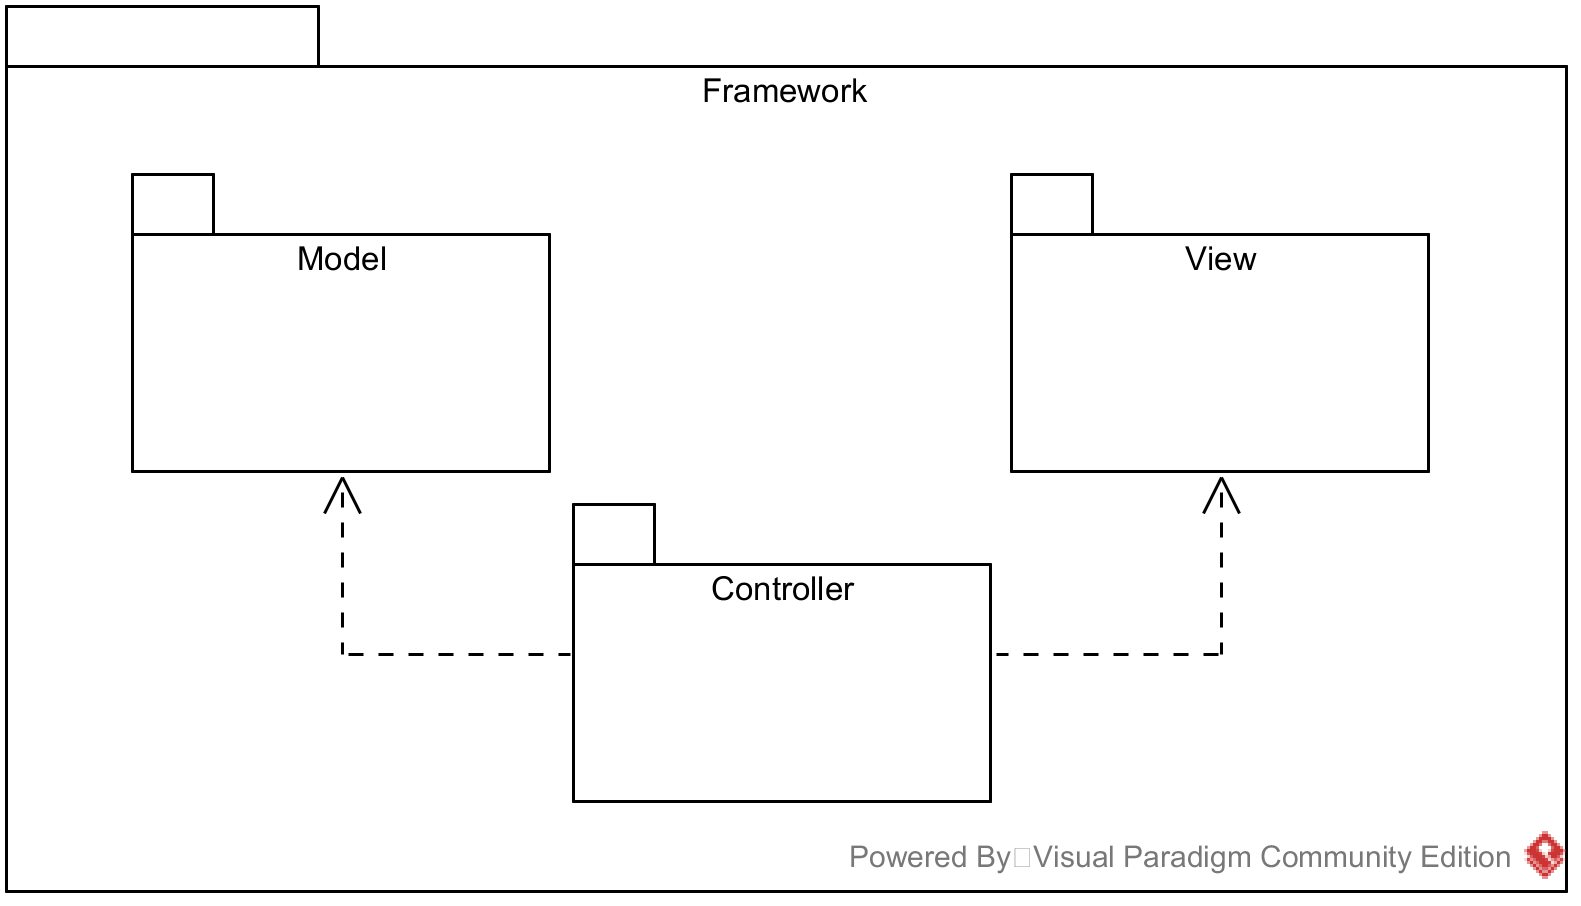
\includegraphics[width=15cm]{./diagrammi/framework.png}
%	\caption{Componente Framework}
%\end{figure}
Il package controller è composto dalla classe listItemActions.

\setclass{TodoList::Controller::listItemActions}
\paragraph[::listItemActions]{\class}\mbox{}\\ \label{\class}
%\begin{figure}[H]
%	\centering
%	\includegraphics[width=15cm]{./diagrammi/demo/todo-list/listitem.png}
%	\caption{Componente Framework}
%\end{figure}
\textbf{Descrizione:}
Questa classe prende le interazioni con l'utente effettuate sulla view e inoltra le richieste al model.

\textbf{Utilizzo:}
Viene utilizzata per comunicare tra la view e il model.

\textbf{Metodi:}
\begin{itemize}
	\item \method{+listItemActions()}: costruttore della classe;
	\item \method{+addItem(text:string)}: comunica al model di inserire un oggetto;
	\begin{itemize}
		\item \param{text:string}: nome dell'oggetto da inserire.
	\end{itemize}
	\item \method{+removeItem(id:string)}: comunica al model di rimuovere un oggetto;
	\begin{itemize}
		\item \param{id:string}: id dell'oggetto da rimuovere.
	\end{itemize}
	\item \method{+completeItem(id:string)}: comunica al model di completare un oggetto.
	\begin{itemize}
		\item \param{id:string}: id dell'oggetto da completare.
	\end{itemize}
\end{itemize}
